\documentclass[11pt,a4paper,twocolumn]{scrartcl}

% Support for UTF-8 and non-English letters require the following two
\usepackage[T1]{fontenc}
\usepackage[utf8]{inputenc}
\usepackage{algorithm2e}
\usepackage{fancyvrb}
% Font packages
\usepackage[default,defaultsans,oldstyle,proportional]{lato}
\usepackage[scaled]{beramono}
\usepackage{sfmath}
% Optimized justification via improved microtypography on character level
\usepackage{microtype}
\usepackage{ragged2e}
\usepackage[none]{hyphenat} % disable all hyphenation
\setlength{\emergencystretch}{3em} % allow extra hfill, needed if hyphenation disabled
%\overfullrule=1mm % mark overfull boxes
%\usepackage{showframe} % show edges of text areas
% Page layout
\usepackage[left=15mm,right=15mm,top=15mm,bottom=20mm,
   nohead,foot=10mm]{geometry}
% Page headers

\usepackage{scrlayer-scrpage}
\usepackage{lastpage}
% Page header
\KOMAoptions{headsepline=0pt,plainheadsepline=off}
\ihead*{}
\chead*{}
\ohead*{}
% Page footer
\KOMAoptions{footsepline=0pt,plainfootsepline=off}
\ifoot*{}
\cfoot*{Page \thepage{} of \pageref*{LastPage}}
\ofoot*{}
% Text layout
\KOMAoption{parskip}{never}
\newlength{\myparindent}
\newlength{\myparskip}
\setlength{\myparindent}{0pt}
\setlength{\myparskip}{5pt plus 1pt}
\setparsizes{\myparindent}{\myparskip}{0.1\linewidth plus 1fil}
\RedeclareSectionCommand[beforeskip=6pt,afterskip=3pt,afterindent=false]{section}
\RedeclareSectionCommand[beforeskip=6pt,afterskip=-0.5em,afterindent=false]{paragraph}
\RaggedRight
% SVN metadata
\usepackage[today,revrange,nofancy]{svninfo}
\svnInfo $Id$
% Graphics
\usepackage{graphicx}
% Colour definitions
\usepackage{xcolor}
\definecolor{secondary}{HTML}{435584}
% Floats
\usepackage{subcaption}
% Listings
\usepackage{listings}
\lstset{language=C, basicstyle=\small\ttfamily,
   aboveskip=0pt, belowskip=0pt}
\usepackage{upquote} % to use correct glyphs for single-quote in verbatim
% SI units
\usepackage{siunitx}
\sisetup{per-mode = symbol, detect-all = true}
% Hyperlinks
\usepackage[
   colorlinks=true,allcolors=secondary,breaklinks=true,
   bookmarks=true,unicode=true,bookmarksopen,bookmarksnumbered]{hyperref}
\usepackage{multicol}

% Package for pseudocode.
\usepackage{algorithm2e}
% Package for inline, verbatim text (code snippets)
\usepackage{fancyvrb}
% Math environments, including align(*)
\usepackage{amsmath}

% Document-specific settings
\renewcommand\abstractname{Executive Summary}

% define a critical section block
\SetKwBlock{CritSection}{critical section}{}

% Document details
\title{Design Brief: Group 5}
\author{
   Gabriel Apap,
   Damjan Filipovic,
   Mark Mizzi
   }
\date{\svnMaxToday, Document v.\svnInfoMaxRevision}

\hypersetup{
   colorlinks   = true
}

\begin{document}

\maketitle

\abstract{%
   This document outlines the design of a DTMF encoding system based on a microcontroller board. The system described makes use of an LCD display to show the user what keys they have pressed as well as to display any messages or errors. An LED is used as an indicator of the system's state. An on-board DAC, in conjunction with an amplifier circuit and speaker are used to generate and amplify the DTMF tones.
   }

\section{Introduction}

   Dual Tone Multi Frequency (DTMF for short) encoding is a technology used to communicate with other devices over a standard analogue telephone line \cite{sl:an218}. This is mainly used for automated switchboards for calls; however, this is also used in remote control systems, telephone banking, and other applications \cite{sl:an218}.

   The technology functions by converting each of the 16 symbols on a keypad (1-9, A-D, * and \#) into a specific tone. The tone consists of a sum of two sine waves, whose frequency is determined by pairwise combination of 4 high frequencies (representing the keypad columns) and 4 low frequencies (representing the keypad rows) \cite{sl:an218}.

   The goal of this project is to implement a DTMF encoding system based on the Embedded Artists LPC4088 microcontroller board.

   Microcontrollers are designed for use in real-time systems, and hence their software stack typically does not include an operating system. Task scheduling has to be handled explicitly by the programmer, through the use of an ad-hoc scheduler and/or interrupt handlers.

   In addition, microcontrollers are generally low-cost systems with limited hardware resources, and hence require the use of low-level programming tricks to achieve efficiency and performance despite the resource constraints.
   
   The DTMF system implemented makes use of several I/O devices, including an LCD used to convey user input or settings options to the user,
   an indicator LED which turns on when the system is booted, and a keypad input device used to navigate menus or to input DTMF symbols.

   The system also has a rich user interface which offers several options. This interface is illustrated in the control flow diagram of Figure~\ref{fig:system-interface}, and will now be described.

   On boot-up, the system prompts the user to enter one of three operational modes: manual mode, quickdial mode, and settings mode.

   In manual mode, the user can input DTMF tones on the keypad, which displays the corresponding symbol on the LCD screen, and plays the appropriate DTMF tone using the DAC and attached amplifier/speaker circuit.

   In settings mode, the user is allowed to set values for the following system parameters:
   \begin{enumerate}
      \item intersymbol spacing, i.e. the delay between two consecutive tones being produced. Has maximum and minimum values of $0$ and $5000$ ms respectively. The default value is $200$ ms.
      \item Symbol length, i.e. the duration for which a single tone is produced. Has maximum and minimum values of $50$ and $5000$ ms respectively. The default value is $500$ ms.
      \item Quality. This setting affects how faithful the tones produced by the system are to a DTMF tone proper. The trade-off involves efficiency, so a higher quality setting results in more power consumption (more CPU activity). Has maximum and minimum values of $4$ and $9$ respectively. The default value is $5$. The exact relationship between this quality value and the precision of the tone produced is discussed below.
   \end{enumerate}

   The user's selected values are validated, and persisted to EEPROM, so that a reboot of the system does not erase its configuration. Values which fall outside of a valid range are rejected, and the corresponding system parameter is set to a default value instead of the user's selection.

   After modifying a system parameter, the user is redirected to boot mode, and can continue using the system as they please.

   In quickdial mode, the user is allowed to create, playback, or delete one of $10$ profiles assigned to each of the numeric ($0-9$) keys. Each profile can store up to $32$ DTMF symbols, and includes its own system configuration (with custom values for each of the three system parameters above). These profiles could be used to communicate with DTMF decoders which expect a certain sequence of symbols, and have constraints on the intersymbol spacing, symbol length, and quality required for decoding.

   \begin{figure*}
      \centering
      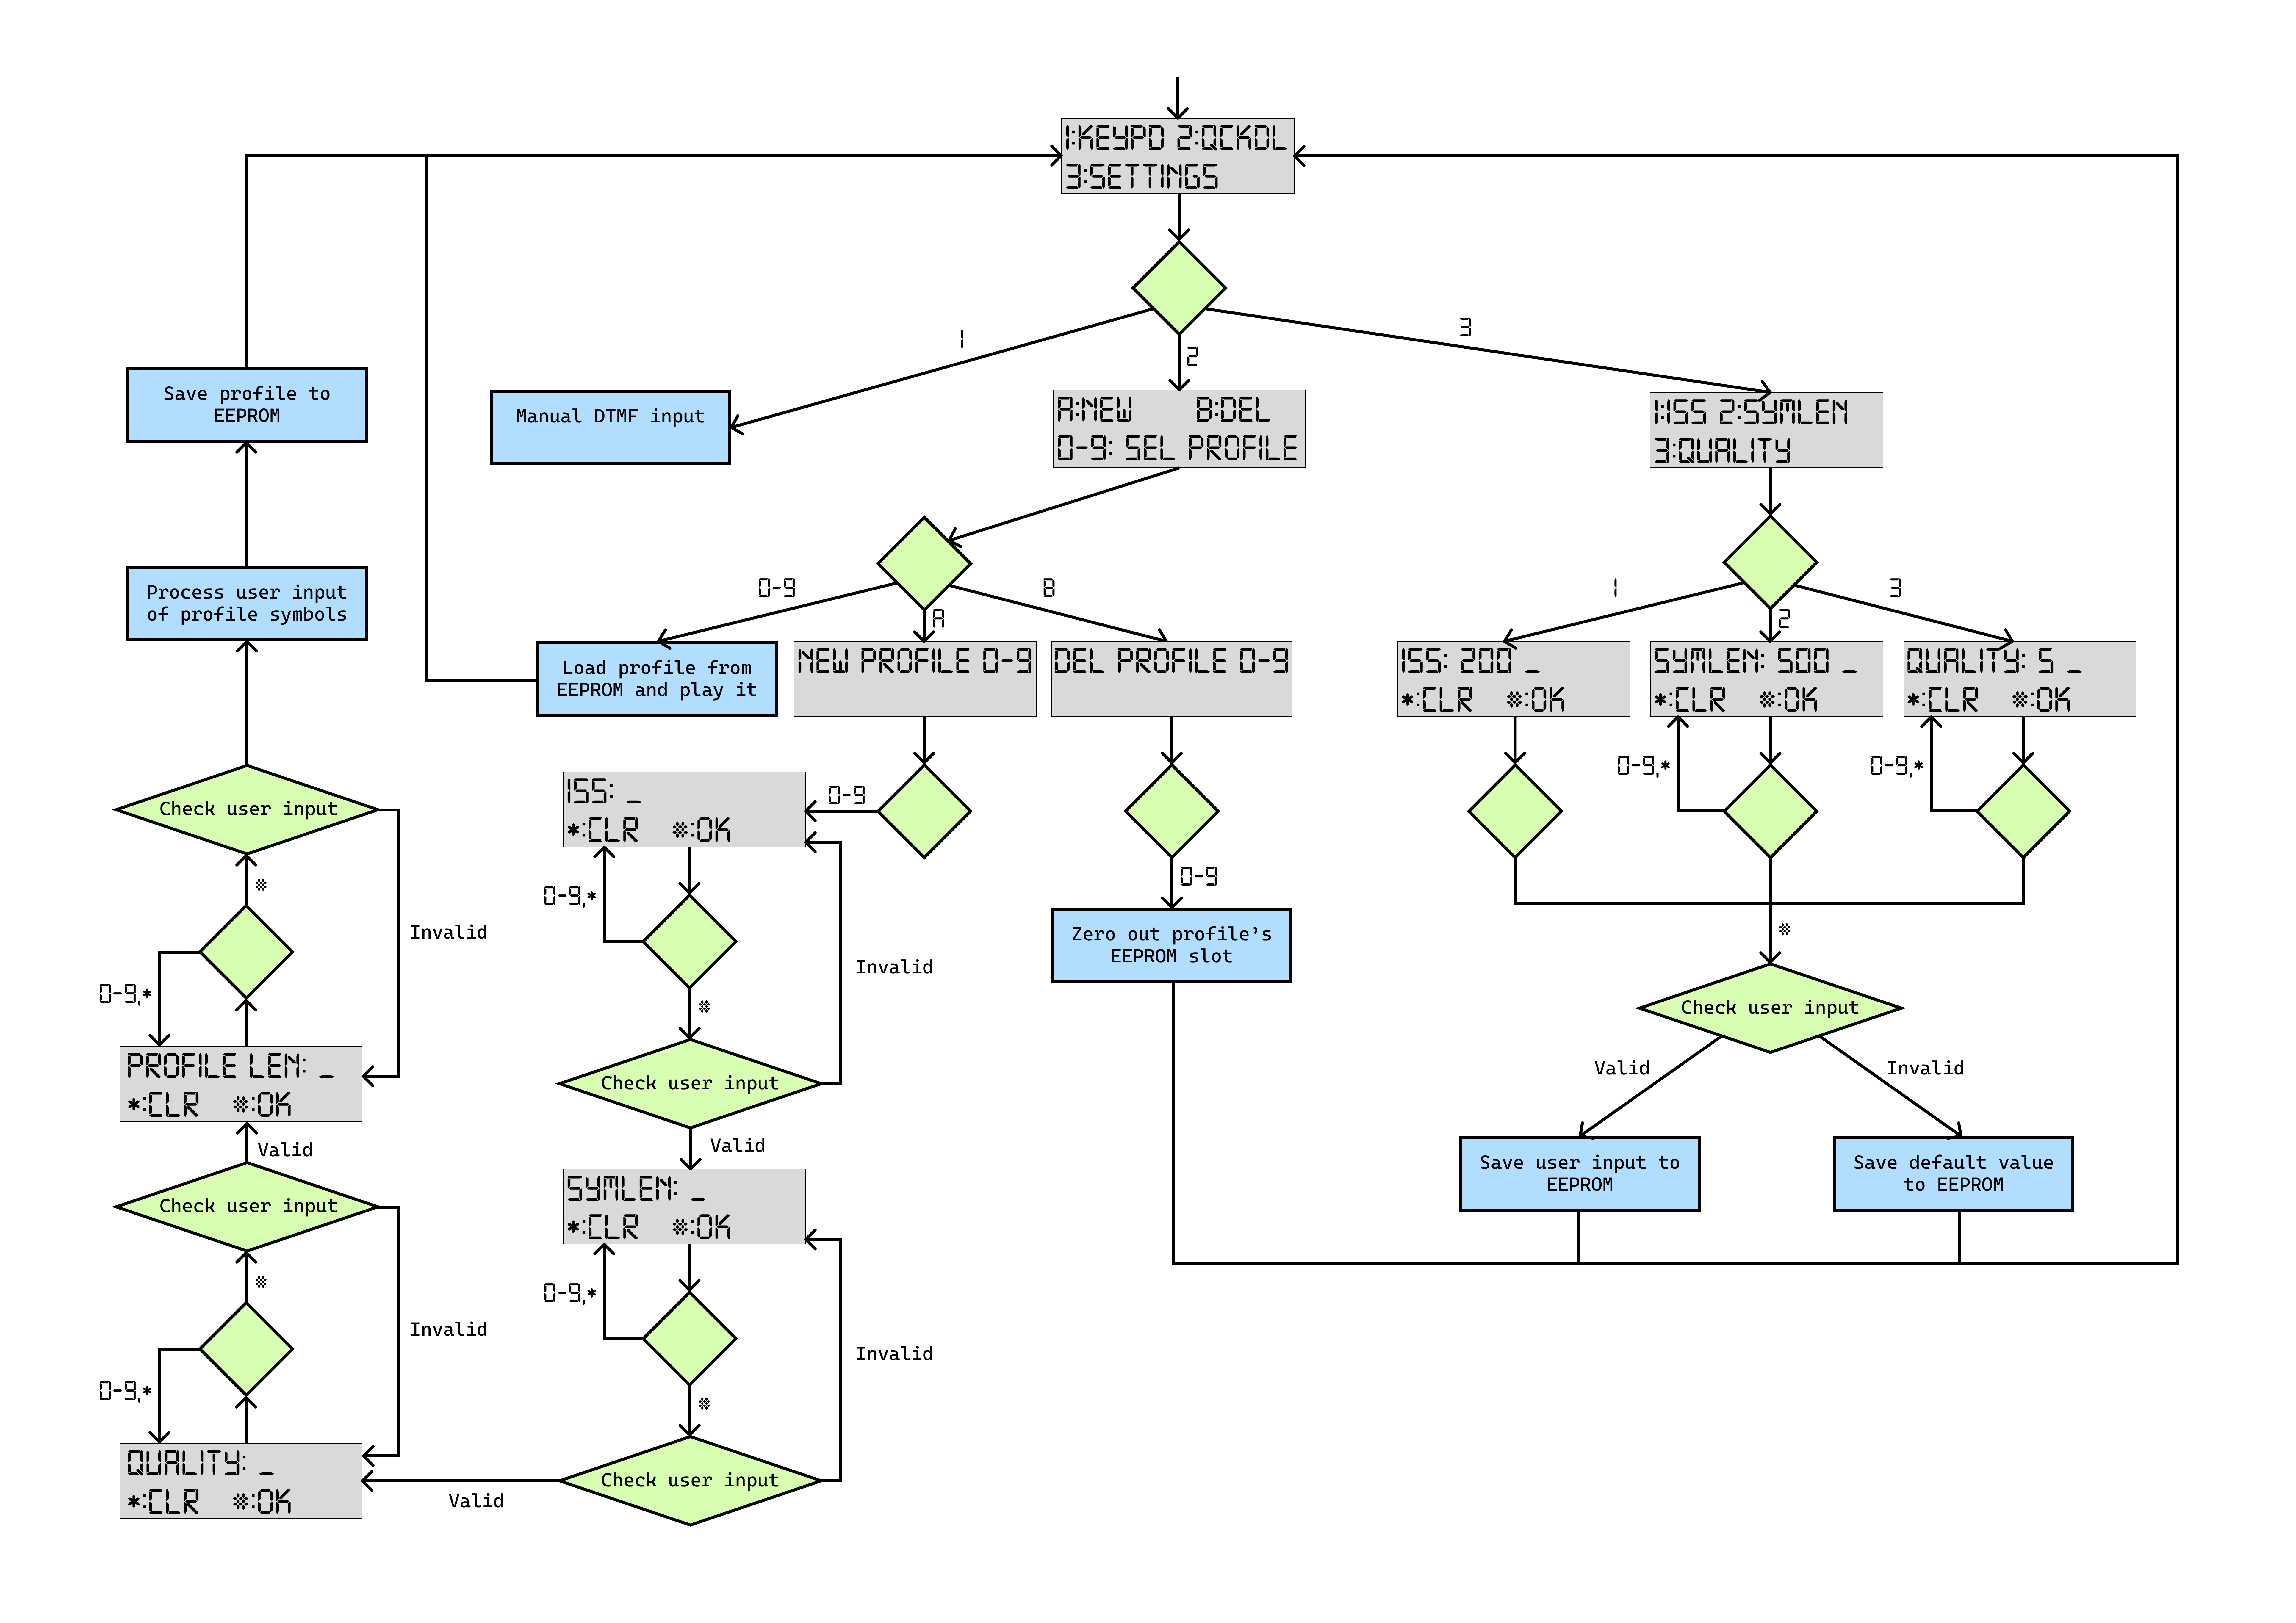
\includegraphics[height=0.67\textheight, angle=90]{system_flow_chart}
      \caption{Flow chart showing system interface. Grey boxes represent the contents of the LCD screen as displayed to the user. Some system actions, such as clearing/displaying user input are omitted for brevity. Keypad input which is ignored by the system is also omitted.}~\label{fig:system-interface}
   \end{figure*}

   Excluding some initial setup, the system is entirely interrupt-based, and the CPU is inactive (in sleep mode) while no interrupt is being handled. This approach was found to result in a significant reduction of power consumption. TODO: Actual numbers.

   Section \ref{system-design} describes the design of the DTMF encoding system. The system's architecture and separation of concerns is described in subsection \ref{system-arch}. Subsection \ref{dac} describes the implementation of DTMF tone generation. Subsection \ref{keypad} discusses how keypad input is handled. Finally, subsection \ref{settings-quickdial} describes how settings and quickdial are implemented, including the use of EEPROM as a persistent storage medium.

   Section \ref{schedule} outlines a breakdown of the system's implementation into individual tasks, as well as a schedule for implementing these tasks.

\section{System Design}~\label{system-design}

\subsection{System architecture}~\label{system-arch}

To implement a variety of features while adhering to good seperation of concerns, the system makes use of several software components. Code for these components is grouped into one or more source files. These software components, together with their constituent source files are shown in Figure \ref{fig:software_components}.

\begin{figure*}
   \centering
   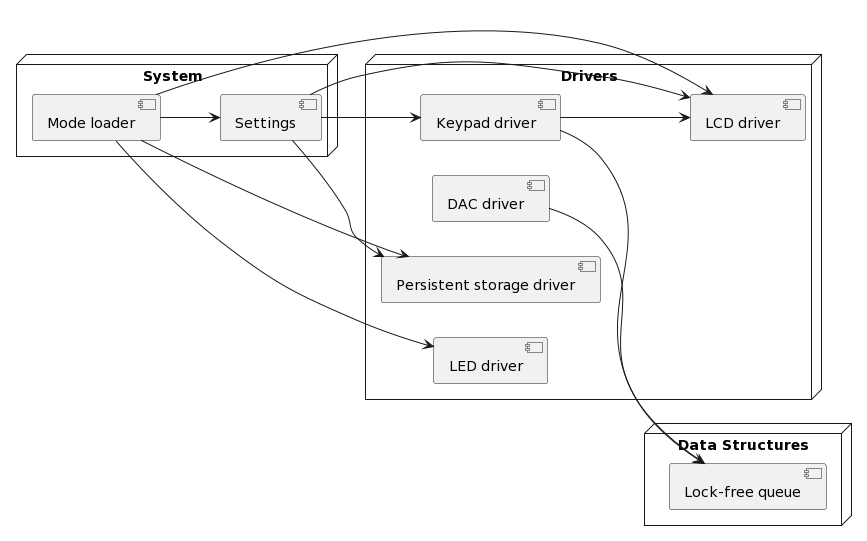
\includegraphics[width=0.92\textwidth]{software_components}
   \caption{Software components for the system. The source files constituting each component are also shown.}
   \label{fig:software_components}
\end{figure*}

The drivers component includes all code that interacts with the board's hardware in a low level way (manipulation of hardware registers). A large portion of this code is sourced from other projects, and adapted for use in our system. Notably, the EEPROM driver was sourced from \href{https://github.com/RT-Thread/realboard-lpc4088/tree/master/software/lpcware_lpc408x/Drivers}{this project}.

The utilities component contains functions for busy waiting a fixed number of milliseconds, or microseconds. These are used in the LCD driver, as well as for software de-bouncing while processing keypad input (see below).

The LCD component provides a high level interface for interacting with the LCD.

The tone generation component contains code that is used to generate samples for the DTMF tones. It also contains a global thread-safe queue which is used to enqueue symbols entered in the keypad, as well as functions which can start the generation of a tone, or enqueue its symbol for later processing. The component is used by quickdial code, as well as in the manual mode of the system.

The keypad component contains code for processing keypad input. This includes an interrupt service routine that is executed when a key press is detected, a function for initializing the GPIO pins used by the keypad, as well as another for customizing the callback called when a key press is registered. The component is used by all system modes to process user input.

The menu component contains utility functions that are used to build menus in settings and quickdial mode, as well as for processing numerical user input.

The settings and quickdial components contain code for each of the two respective modes.

\subsection{DTMF tone generation}~\label{dac}

This section describes the design of code in the tone generation component mentioned above.

Tones are produced using a function called \verb!tone_play_or_enqueue!. 

This function takes a DTMF symbol (in the form of a column and a row), and attempts to start generating its tone by calling another function \verb!dac_interrupt_enable!.

\verb!dac_interrupt_enable! returns a boolean to indicate success or failure. It will fail if another DTMF tone is currently being produced by the system, and succeeds otherwise.

Given that the maximum symbol length and intersymbol spacing are $5$s each, a user can easily enter symbols faster than their tones are produced, and hence the failure of \verb!dac_interrupt_enable! is a common situation that the system has to deal with.

On failure, our system enqueues the symbol passed to \verb!tone_play_or_enqueue! to a global queue, and this is later dequeued by the timer ISR generating the tone when it is done.

The salient point in this discussion is that the system uses a global queue which can be concurrently accessed by consumers and producers (due to interleaving of multiple ISRs and normal code).

To meet the system's needs, the queue needed to support the following operations:
\begin{enumerate}
   \item Enqueue a DTMF symbol.
   \item Check if queue is empty and dequeue. This must be one atomic operation.
\end{enumerate}

Due to concurrent access, the queue also had to be implemented with thread safety in mind, i.e. its operations had to be atomic. However, some simplifying assumptions were made in implementing this queue.

Firsly, concurrent execution of two producers is not possible. In manual mode, tones are enqueued by a GPIO ISR, and since one GPIO ISR cannot preempt another, enqueuing occurs serially in this case. Similarly, in quickdial mode, tones are enqueued in normal mode, and hence the producer code is serial.

Concurrent execution of two consumers is also not possible. Symbols are dequeued by timer ISRs running on a single timer peripheral. It is easy to see that timer interrupts that invoke these ISRs can only happen serially.

Secondly, a fixed size queue was deemed acceptable. This assumption allows us to implement the queue as a circularly indexed array, rather than a more complex linked list data structure. A size of 2048 elements was chosen.

To see why this approach is acceptable, consider the worst case scenario, where both intersymbol spacing and symbol length are each set to their maximum values of $5$s, so that processing of a single symbol takes $10$s. 

It is safe to assume that the most eager user would enter key presses at a rate of not more than $3$ symbols per second. This means that symbols are enqueued at an overall rate of $3 - 1/10 = 2.9$ symbols per second. For the queue to overflow, the user has to continuously enter input for $2048/2.9 = 706$ seconds, or more than $11$ minutes.

This was deemed to be an unlikely situation. Note however, that were the queue to overflow, there would not be a catastrophic failure of the system; instead the oldest entered symbols would simply be discarded.

Although this implementation approach significantly simplifies code, and may also be more performant than a linked list approach (which would resort to a \verb!malloc! implementation for allocating nodes), one downside is that the statically allocated queue takes up a significant portion of memory, while being mostly under-utilized.

The thread safe queue operations were implemented using hardware synchronization. The ARMv7-M architecture provides \verb!LDREX! (load exclusive) and \verb!STREX! (store exclusive) instructions for this purpose.

When a load exclusive instruction is used, a hardware monitor tracks subsequent stores to a small block containing the loaded address using a tag. Once a single exclusive store to the block has been executed, the monitor prevents subsequent exclusive stores before another exclusive load is performed.\cite{armv7_m_architecture_manual}

The use of these instructions required the queue to be implemented in ARM assembly (inline assembly is discouraged when using exclusive load/store instructions).

Pseudo-code for the two operations implemented is shown in Listing~\ref{alg:enqueue} and Listing~\ref{alg:check_dequeue} respectively. A line marked as \textbf{atomic}, or a section marked \textbf{critical-section} indicate code which is protected by \verb!LDREX!/\verb!STREX! guards. Note also that thread safety can be achieved simply by guarding access to a single, additional shared variable; the queue size. This is possible because there is only one producer and one consumer that concurrently access the queue, so it is impossible for the queue's head or tail index variables to be shared.

\begin{algorithm}
   \caption{Pseudocode for the lock-free queue's enqueue operation. Note the atomic increment of $N$}\label{alg:enqueue}
   \KwData{
      \begin{itemize}
         \item $q$ is the queue array
         \item $tail$ is the immediate index after the last element in the queue
         \item $s$ is the symbol to be enqueued
         \item $N$ is the number of items in the queue
         \item $M$ is the queue size (maximum capacity of the queue)
      \end{itemize}}
      \textbf{atomic} $N \gets (N + 1) \bmod M$; \\
      $q[tail] \gets s$; \\
      $tail \gets (tail + 1) \bmod M$;
\end{algorithm}

\begin{algorithm}
   \caption{Pseudocode for the lock-free queue's check and dequeue operation.}\label{alg:check_dequeue}
   \KwData{
      \begin{itemize}
         \item $q$ is the queue array
         \item $head$ is the index of the start of the queue
         \item $N$ is the number of items in the queue
         \item $M$ is the queue size (maximum capacity of the queue)
         \item $default$ is the smallest integer value ($-2^{31}$).
      \end{itemize}}
      \CritSection{
         $tmp \gets N$;\\
         \If{$tmp = 0$}
         {
             $N \gets (tmp - 1) \bmod M$\;
         }
      }
      $res \gets default$;\\
      \If{$tmp \ne 0$}
      {
         $res \gets q[head]$;\\
         $head \gets (head + 1) \bmod M$;
      }
\end{algorithm}

There is one more place where the system requires considerations of thread safety. In \verb!dac_interrupt_enable!, the code requires a way of knowing whether a tone is playing or not, in order to succeed or fail in starting the next tone. For this purpose, a global variable \verb!dac_interrupt_flag! is used. This flag is set when a timer interrupt is enabled, and reset when one is disabled.

However, when \verb!dac_interrupt_enable! checks the global flag, the following data race can occur:
\begin{enumerate}
   \item First, \verb!dac_interrupt_flag!, which happens to have a value of $1$, is loaded from memory into a register.
   \item Next, the thread of execution running \verb!dac_interrupt_enable! is preempted by a timer interrupt.
   \item The timer ISR invoked happens to be the one at the end of tone generation. It checks the queue, which happens to be empty, resets \verb!dac_interrupt_flag! and exits.
   \item \verb!dac_interrupt_enable! continues executing with the wrong value for \verb!dac_interrupt_flag!, resulting in an unneeded failure.
\end{enumerate}

This sequence of events will prevent a tone from being generated for the entered symbol. Instead, it is enqueued, and its tone may be produced after the next entered symbol is processed.

In order to prevent this data race, \verb!dac_interrupt_flag! is accessed using an atomic test-and-set in \verb!dac_interrupt_enable!. This is again implemented using a \verb!LDREX/STREX! pair.

DTMF tones consist of a composition of two sine waves whose frequency is determined by the row and column index of the corresponding DTMF symbol.

The sine function is fairly computationally intensive, and hence our system precomputes samples for one period of a sine wave, storing them in a lookup table. The table is filled in each time the system enters manual mode, or loads a quickdial profile. The number of samples in the table is determined by the quality setting, which is log base $2$ of the size. This means that the size ranges from $16$ to $512$ samples. The exact relationship between the size of the lookup table and the quality of the tone produced will be discussed below.

In what follows, $LUT$ represents the lookup table, $N$ its size, and $f_1$ and $f_2$ are the higher and lower frequencies of a DTMF tone.

In order to make the most efficient use of the sine lookup table, the frequency of the timer interrupt is set to $4$ times the highest frequency of the DTMF tone being produced. This means that one of the sine waves can be produced simply by repeatedly getting the $0$th, $N/4$th, $N/2$th and $3N/4$th samples from the lookup table in each invocation of the ISR. 

Note that since the DTMF tone signal has a frequency spectrum bandlimited by $f_1$, the Nyquist criterion specifies that the lower bound on the sampling frequency of the signal should be $2f_1$. In this case, we are using a sampling frequency of $4f_1$, which is fairly close. The relationship between sampling frequency and $f_1$ was determined empirically.

Samples for the lower frequency sine component of the DTMF tone are determined using the following formula:
$$ \frac{1}{2}\Bigg(LUT\bigg[\bigg\lfloor\frac{f_2i}{f_1}\bigg\rfloor \bmod N\bigg] + LUT\bigg[\bigg\lceil\frac{f_2i}{f_1}\bigg\rceil \bmod N\bigg]\Bigg) $$
where $i$ is a global variable (called \verb!sample_index! in the code) which keeps track of the tone generation progress in between timer ISR invocations, and is incremented by $N/4$ each time the timer ISR is invoked.

The formula above essentially finds the two samples that lie on either side of the sine value required, and then averages them. This is why increasing the size of the lookup table improves the quality of the tone produced; it improves the precision of the result computed by this average.

One note about implementation; regular integer division is the floor of the real result when the latter is positive, as in the above case. Ceiling division is accomplished using the following formula\cite{warren2012hacker}:
$$ \bigg\lceil \frac{x}{y} \bigg\rceil = -\bigg\lfloor -\frac{x}{y} \bigg\rfloor $$

A number of optimizations were applied to the formula for the lower frequency sine component. Firstly, $N$ is fixed to be a power of $2$ (recall that the quality setting is $\log_2 N$), and hence the modulo operation can be replaced by a bitwise and, using the following formula that works when $y$ is a power of two:
$$ x \bmod y = x \,\,\&\,\, (y - 1) $$

Secondly, the two divisions by $f_1$ are costly, but avoidable. By having one version of the timer ISR for each possible tone, the divisions become constant, allowing them to be optimized into a shift and a multiplication by the compiler\cite{warren2012hacker}. In order to implement this specialization cleanly, \verb!timer_callback_isr! is declared as \verb!STATIC_INLINE! (encouraging the compiler to inline its body), and macros are used to define specialized wrappers for it, for example \verb!timer_callback_isr_1209_697!. Function pointers to these specialized wrappers are stored in a 2-dimensional \verb!dispatch_table! variable, with the pointer at a particular 2-dimensional index pointing to the wrapper that produces the tone with the corresponding row and column index. This arrangement has additional benefits, namely the elimination of global state that would have to keep track of what tone is being produced in between invocations of the timer ISR.

Earlier, it was mentioned that the timer ISR checks if tone generation has finished, and attempts to start generating a new tone if this is the case. This is done at the end of \verb!timer_callback_isr!, by comparing the value of \verb!sample_index! with $f_1 \times N \times \text{symbol length in seconds}$.

If the latter check succeeds, the tone has been generated for the duration determined by the system's symbol length setting, and \verb!timer_callback_isr! calls \verb!timer_set_callback_delay!. This function takes a callback and a delay (in CPU cyles), and sets up the timer to call this callback after the given delay. Since the same timer peripheral is used for driving the DAC and for the delayed callback, this call simultaneuosly disables \verb!timer_callback_isr! from being invoked again. The callback in this case is \verb!pop_and_dac_interrupt_enable!.

This function dequeues any existing symbol in the queue, and enables generation of its tone. Since it is only used by \verb!timer_callback_isr!, there is no need to check \verb!dac_interrupt_flag!, as it must be set when the function is called. Hence the function enables generation of the tone by calling \verb!dac_interrupt_enable_unsafe!, a version of \verb!dac_interrupt_enable! that skips checking or setting \verb!dac_interrupt_flag!. (Since \verb!dac_interrupt_enable_unsafe! is a subset of \verb!dac_interrupt_enable!'s functionality, the latter function wraps the former.) 

%If the queue is empty, the function calls \verb!dac_interrupt_disable!, which resets \verb!dac_interrupt_flag! and disables the timer.
%
%The behaviour of each interrupt handler is shown in the control flow diagram in Figure \ref{fig:tone_interrupt_cfd}.
%
%\begin{figure*}
%   \centering
%   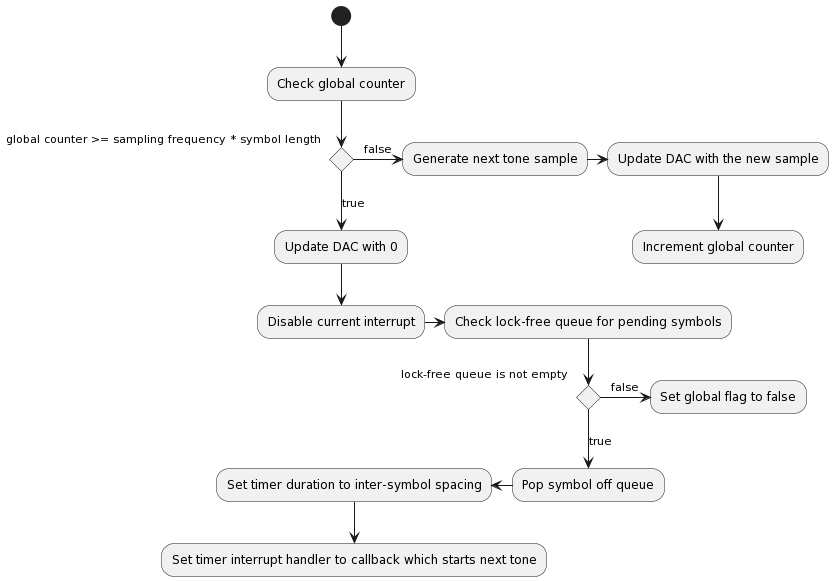
\includegraphics[width=0.92\textwidth]{tone_interrupt_cfd}
%   \caption{Control flow diagram illustrating behaviour of tone-generating interrupt handlers}
%   \label{fig:tone_interrupt_cfd}
%\end{figure*}
%
%The \textbf{keypad driver} component provides an abstraction layer over the keypad. It must implement a single polling cycle (as a function) for use in other modules.
%
%In addition, it must implement a method that whilst running the polling cycle, performs the following actions immediately on detection of a key press:
%\begin{enumerate}
%   \item It immediately outputs the DTMF symbol detected to the LCD screen.
%   \item It checks if there is a tone interrupt handler enabled. This can be done by atomic test and set on the global flag.
%   \item If there is no tone interrupt handler enabled, it takes the symbol detected, and enables a tone-generating interrupt handler to generate its tone 
%      (using a method in the DAC driver).
%   \item If there is already a tone interrupt handler enabled, it pushes the DTMF symbol onto the output queue.
%\end{enumerate}
%This method will be used in normal mode to process key presses.
%
%The \textbf{persistent storage driver} provides an abstraction layer over the flash memory. It provides functions to serialize and deserialize the C structs 
%which need to be stored into a byte stream, and allows for loading or storing serialized data from/to flash memory. The use of a wear leveling algorithm when storing data is essential to prevent the flash memory from degrading quickly\cite{silberschatz2018operating}.

%The \textbf{LED driver} provides methods to turn the indicator LED on or off.
%
%The \textbf{LCD driver} provides an abstraction layer over the LCD screen. It must implement methods which allow a DTMF symbol or a C string to be encoded and
%displayed on the LCD.
%
%
%There are several ways in which the polling cycle procedure that processes user input in normal mode (described above) can be executed.
%
%The simplest method is to run the procedure in application mode, with a set period of busy waiting in between invocations of the method to avoid spurious input.
%(A human user will keep a key pressed for several clock cycles.)
%
%A more sophisticated option is to run the procedure as an interrupt handler for a timer interrupt, with the timer duration set to avoid spurious input. In this version, the processor has no application code to run and can be put in sleep mode in between interrupt invocations. While more efficient than the busy-waiting approach, this method can still invoke the interrupt handler when there is no input to process.

%A final, more efficient approach is to have a keypad-driven interrupt handler. In this approach, the columns of the keypad are set high, and pressing any key
%triggers a pin interrupt for its row. The interrupt handler then invokes the polling method to find which key in that row was pressed and handle it.
%
%Each of these design choices is more sophisticated than the last, while re-using much of the same code. The plan is to implement each of these designs in turn. When one implementation has been successfully tested, the team will move on to implementing a more sophisticated design.

\subsection{Keypad input} \label{keypad}

\subsection{Settings and Quickdial} \label{settings-quickdial}

\section{Management} \label{schedule}
\subsection{Final Deadline}
The final deadline will be set to \textbf{10\textsuperscript{th} May} to ensure that the work is done at a proper pace whilst leaving enough room for any necessary 
adjustments.

\subsection{Tasks}
To implement the system, the above-mentioned software components have to be split into multiple sub-tasks. Each task will have a fairly allocated time-frame for completion. The deadlines for each task are as follows:
\subsubsection{Drivers}
\begin{enumerate}
    \item LCD Driver - Deadline: \textbf{8\textsuperscript{th} April}. Subtasks: Symbol and C-String to LCD function, Display function.
    \item Keypad Driver - Deadline: \textbf{8\textsuperscript{th} April}. Subtasks: Polling Cycle function for the keypad, Keypad driven interrupt.
    \item LED Driver - Deadline: \textbf{8\textsuperscript{th} April}. Subtasks: LED On function, LED Off function.
    \item Persistent Storage Driver - Deadline: \textbf{16\textsuperscript{th} April}. Subtasks: Serialising Data, Persisting Data, Loading Data, Deserializing Data.
    \item DAC Driver - Deadline: \textbf{20\textsuperscript{th} April}. Subtasks: Timer interrupt handler enable method, Set timer duration function, Interrupt handlers.
\end{enumerate}

\subsubsection{Data Structures}
\begin{enumerate}
    \item Lock-Free queue - Deadline: \textbf{1\textsuperscript{st} April}. Subtasks: Atomic Enqueue function, Atomic Check and Dequeue function.
\end{enumerate}

\subsubsection{System}
\begin{enumerate}
    \item Mode loader - Deadline: \textbf{16\textsuperscript{th} April}. Subtasks: Display Options function, Load settings/normal mode functions.
    \item Settings Mode - Deadline: \textbf{27\textsuperscript{th} April}. Subtasks: Display settings function, Save settings function.
\end{enumerate}

\subsection{Task Dependencies}
When considering the inter-dependencies of the tasks listed above, there is a discrete order of task development that when followed should ensure that each subsequent task has adequate resources to be accomplished. The order is the following:
\begin{enumerate}
    \item Lock-Free Queue
    \item LCD Driver
   \item LED Driver
   \item Keypad Driver
   \item Persistent Storage Driver
   \item DAC Driver
\end{enumerate}

\section{Closure}

In conclusion, this document describes the design of an efficient and performant system implementing DTMF encoding. The system's software has been split up
into several modules showing good separation of concerns. Although not discussed here, a highly efficient algorithm has been derived for use in tone generation.

\bibliographystyle{ieeetr}
\bibliography{references}

\end{document}
